\newpage
\chapter{Приближени пресмятания - подходи, методи, алгоритми}
\label{chapter10}
\thispagestyle{empty}

В изчислителната математика се открояват две основни направления – точните числени пресмятания и приближените числени пресмятания\index{приближени пресмятания}. Точни числени пресмятания\index{точни числени методи} се извършват в ситуации в които обемът на задачата позволява изчисленията да се осъществят в приемлив интервал от време. В реалната практика често поставяните задачи значително нарастват като обем и тяхното пресмятане с точени числени методи става неприемливо по отношение на нужното време за пресмятане. В такива ситуации се прибягва до множеството разработени методи за приближени пресмятания\index{приближени числени методи}. По отношение на програмния продукт R, ще бъдат разгледани някои от най-популярните методи за приближени числени пресмятания, а именно Монте-Карло симулации, генетични алгоритми и изкуствени невронни мрежи.

\section{Монте-Карло методи}

В средата на XX век, във връзка с разработването на първите ядрени оръжия, са разработени група методи за приближени пресмятания, които залагат на способ за генериране на голямо количество случайни числа и последващата им статистическа обработка. Монте-Карло методите намират най-голямо приложение в оптимизационни задачи, числено интегриране и генериране на семпли за специфични вероятностни разпределения. Монте-Карло методите могат да се използват за решаването на всяка задача, която има представяне в термините на вероятности и статистика. 

Има вариации в реализацията на Монте-Карло методите, но те в общия случай следват няколко добре дефинирани стъпки:

1. Определяне на област от допустими стойности;

2. Генериране на извадка от случайни числа в предварително дефинираната област;

3. Извършване на точни пресмятания с така генерираните случайни числа;

4. Обобщаване на резултатите от извършените пресмятания.

\begin{figure}[h!]
  \centering
  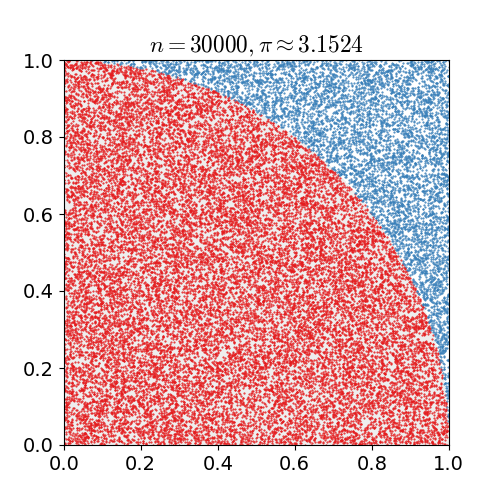
\includegraphics[width=0.8\linewidth]{pic0060}
  \caption{Пресмятане на числото $\pi$ с Монте-Карло метод}
\label{figure0060}
\end{figure}
\FloatBarrier

Един от най-популярните примери за Монте-Карло пресмятане е приближеното изчисление на числото $\pi$ (Фиг. \ref{figure0060}). За тази цел една четвърт от окръжност се представя с обгръщащия я квадрат. Съотношението между площите на квадрата и на четвъртината окръжност е $\pi/4$. За да се апроксимира стойността на числото $\pi$ с Монте-Карло метод се изпълняват следните стъпки:

1. Изчертаване на квадрат и четвъртина окръжност вписана в него;

2. Генериране на случайни равномерно разпределени числа, като координати (x,y двойки) в описаната допустима област;

3. Изброяване на точките с координати x,y които са на разстояние 1 от центъра на четвърт окръжността; 

4. Съотношението между точките в четвърт окръжността и общия брой точки е $\pi/4$, което умножено по 4 дава приближена стойност за числото $\pi$. 

При тази процедура за приближено пресмятане е важно да се вземат под внимание два много важни фактора:

1. Ако генерираните случайни числа не са равномерно разпределени, това ще доведе до невярна апроксимация за търсената стойност;

2. Генерирането на малък брой координати за точки в дефиниционната област води до ниско надеждна стойност за апроксимация, което означава, че колкото по-голям обем е извадката от случайни числа, толкова по-надеждни резултати за апроксимация.


